\documentclass[twoside]{book}

% Packages required by doxygen
\usepackage{calc}
\usepackage{doxygen}
\usepackage{graphicx}
\usepackage[utf8]{inputenc}
\usepackage{makeidx}
\usepackage{multicol}
\usepackage{multirow}
\usepackage{textcomp}
\usepackage[table]{xcolor}

% Font selection
\usepackage[T1]{fontenc}
\usepackage{mathptmx}
\usepackage[scaled=.90]{helvet}
\usepackage{courier}
\usepackage{amssymb}
\usepackage{sectsty}
\renewcommand{\familydefault}{\sfdefault}
\allsectionsfont{%
  \fontseries{bc}\selectfont%
  \color{darkgray}%
}
\renewcommand{\DoxyLabelFont}{%
  \fontseries{bc}\selectfont%
  \color{darkgray}%
}

% Page & text layout
\usepackage{geometry}
\geometry{%
  a4paper,%
  top=2.5cm,%
  bottom=2.5cm,%
  left=2.5cm,%
  right=2.5cm%
}
\tolerance=750
\hfuzz=15pt
\hbadness=750
\setlength{\emergencystretch}{15pt}
\setlength{\parindent}{0cm}
\setlength{\parskip}{0.2cm}
\makeatletter
\renewcommand{\paragraph}{%
  \@startsection{paragraph}{4}{0ex}{-1.0ex}{1.0ex}{%
    \normalfont\normalsize\bfseries\SS@parafont%
  }%
}
\renewcommand{\subparagraph}{%
  \@startsection{subparagraph}{5}{0ex}{-1.0ex}{1.0ex}{%
    \normalfont\normalsize\bfseries\SS@subparafont%
  }%
}
\makeatother

% Headers & footers
\usepackage{fancyhdr}
\pagestyle{fancyplain}
\fancyhead[LE]{\fancyplain{}{\bfseries\thepage}}
\fancyhead[CE]{\fancyplain{}{}}
\fancyhead[RE]{\fancyplain{}{\bfseries\leftmark}}
\fancyhead[LO]{\fancyplain{}{\bfseries\rightmark}}
\fancyhead[CO]{\fancyplain{}{}}
\fancyhead[RO]{\fancyplain{}{\bfseries\thepage}}
\fancyfoot[LE]{\fancyplain{}{}}
\fancyfoot[CE]{\fancyplain{}{}}
\fancyfoot[RE]{\fancyplain{}{\bfseries\scriptsize Generated on Wed Nov 20 2013 16\-:25\-:39 for Srivener\-Capitulos by Doxygen }}
\fancyfoot[LO]{\fancyplain{}{\bfseries\scriptsize Generated on Wed Nov 20 2013 16\-:25\-:39 for Srivener\-Capitulos by Doxygen }}
\fancyfoot[CO]{\fancyplain{}{}}
\fancyfoot[RO]{\fancyplain{}{}}
\renewcommand{\footrulewidth}{0.4pt}
\renewcommand{\chaptermark}[1]{%
  \markboth{#1}{}%
}
\renewcommand{\sectionmark}[1]{%
  \markright{\thesection\ #1}%
}

% Indices & bibliography
\usepackage{natbib}
\usepackage[titles]{tocloft}
\setcounter{tocdepth}{3}
\setcounter{secnumdepth}{5}
\makeindex

% Hyperlinks (required, but should be loaded last)
\usepackage{ifpdf}
\ifpdf
  \usepackage[pdftex,pagebackref=true]{hyperref}
\else
  \usepackage[ps2pdf,pagebackref=true]{hyperref}
\fi
\hypersetup{%
  colorlinks=true,%
  linkcolor=blue,%
  citecolor=blue,%
  unicode%
}

% Custom commands
\newcommand{\clearemptydoublepage}{%
  \newpage{\pagestyle{empty}\cleardoublepage}%
}


%===== C O N T E N T S =====

\begin{document}

% Titlepage & ToC
\hypersetup{pageanchor=false}
\pagenumbering{roman}
\begin{titlepage}
\vspace*{7cm}
\begin{center}%
{\Large Srivener\-Capitulos }\\
\vspace*{1cm}
{\large Generated by Doxygen 1.8.5}\\
\vspace*{0.5cm}
{\small Wed Nov 20 2013 16:25:39}\\
\end{center}
\end{titlepage}
\clearemptydoublepage
\tableofcontents
\clearemptydoublepage
\pagenumbering{arabic}
\hypersetup{pageanchor=true}

%--- Begin generated contents ---
\chapter{Namespace Index}
\section{Packages}
Here are the packages with brief descriptions (if available)\-:\begin{DoxyCompactList}
\item\contentsline{section}{\hyperlink{namespacetreeview_capitulos_personajes}{treeview\-Capitulos\-Personajes} }{\pageref{namespacetreeview_capitulos_personajes}}{}
\end{DoxyCompactList}

\chapter{Hierarchical Index}
\section{Class Hierarchy}
This inheritance list is sorted roughly, but not completely, alphabetically\-:\begin{DoxyCompactList}
\item \contentsline{section}{treeview\-Capitulos\-Personajes.\-Capitulo}{\pageref{classtreeview_capitulos_personajes_1_1_capitulo}}{}
\item \contentsline{section}{treeview\-Capitulos\-Personajes.\-Escena}{\pageref{classtreeview_capitulos_personajes_1_1_escena}}{}
\item Form\begin{DoxyCompactList}
\item \contentsline{section}{treeview\-Capitulos\-Personajes.\-Formulario}{\pageref{classtreeview_capitulos_personajes_1_1_formulario}}{}
\end{DoxyCompactList}
\item \contentsline{section}{treeview\-Capitulos\-Personajes.\-I\-Persistencia}{\pageref{interfacetreeview_capitulos_personajes_1_1_i_persistencia}}{}
\begin{DoxyCompactList}
\item \contentsline{section}{treeview\-Capitulos\-Personajes.\-Xml\-Persistencia}{\pageref{classtreeview_capitulos_personajes_1_1_xml_persistencia}}{}
\end{DoxyCompactList}
\item \contentsline{section}{treeview\-Capitulos\-Personajes.\-I\-Tree\-Lateral}{\pageref{interfacetreeview_capitulos_personajes_1_1_i_tree_lateral}}{}
\begin{DoxyCompactList}
\item \contentsline{section}{treeview\-Capitulos\-Personajes.\-Formulario}{\pageref{classtreeview_capitulos_personajes_1_1_formulario}}{}
\end{DoxyCompactList}
\item \contentsline{section}{treeview\-Capitulos\-Personajes.\-Libro}{\pageref{classtreeview_capitulos_personajes_1_1_libro}}{}
\item \contentsline{section}{treeview\-Capitulos\-Personajes.\-Personaje}{\pageref{classtreeview_capitulos_personajes_1_1_personaje}}{}
\item \contentsline{section}{treeview\-Capitulos\-Personajes.\-Ppal}{\pageref{classtreeview_capitulos_personajes_1_1_ppal}}{}
\end{DoxyCompactList}

\chapter{Class Index}
\section{Class List}
Here are the classes, structs, unions and interfaces with brief descriptions\-:\begin{DoxyCompactList}
\item\contentsline{section}{\hyperlink{classtreeview_capitulos_personajes_1_1_capitulo}{treeview\-Capitulos\-Personajes.\-Capitulo} \\*Clase que almacena la informacion relativa a un capitulo del libro. }{\pageref{classtreeview_capitulos_personajes_1_1_capitulo}}{}
\item\contentsline{section}{\hyperlink{classtreeview_capitulos_personajes_1_1_escena}{treeview\-Capitulos\-Personajes.\-Escena} \\*Clase que representa las escenas que componen los capitulos del libro. }{\pageref{classtreeview_capitulos_personajes_1_1_escena}}{}
\item\contentsline{section}{\hyperlink{classtreeview_capitulos_personajes_1_1_formulario}{treeview\-Capitulos\-Personajes.\-Formulario} \\*Esta es la clase encargada de dibujar el win\-Form con el treeview. }{\pageref{classtreeview_capitulos_personajes_1_1_formulario}}{}
\item\contentsline{section}{\hyperlink{interfacetreeview_capitulos_personajes_1_1_i_persistencia}{treeview\-Capitulos\-Personajes.\-I\-Persistencia} \\*Esta interfaz representa a la persistencia permitiendo su utilización sea cual sea su implementacion. }{\pageref{interfacetreeview_capitulos_personajes_1_1_i_persistencia}}{}
\item\contentsline{section}{\hyperlink{interfacetreeview_capitulos_personajes_1_1_i_tree_lateral}{treeview\-Capitulos\-Personajes.\-I\-Tree\-Lateral} \\*Interfaz que permite el uso de una interfaz grafica de forma transparente. }{\pageref{interfacetreeview_capitulos_personajes_1_1_i_tree_lateral}}{}
\item\contentsline{section}{\hyperlink{classtreeview_capitulos_personajes_1_1_libro}{treeview\-Capitulos\-Personajes.\-Libro} \\*Esta clase contiene toda la informacion necesaria para la creacion de Tree\-View relativa al libro. }{\pageref{classtreeview_capitulos_personajes_1_1_libro}}{}
\item\contentsline{section}{\hyperlink{classtreeview_capitulos_personajes_1_1_personaje}{treeview\-Capitulos\-Personajes.\-Personaje} \\*Contiene la informacion relativa a un personaje. }{\pageref{classtreeview_capitulos_personajes_1_1_personaje}}{}
\item\contentsline{section}{\hyperlink{classtreeview_capitulos_personajes_1_1_ppal}{treeview\-Capitulos\-Personajes.\-Ppal} }{\pageref{classtreeview_capitulos_personajes_1_1_ppal}}{}
\item\contentsline{section}{\hyperlink{classtreeview_capitulos_personajes_1_1_xml_persistencia}{treeview\-Capitulos\-Personajes.\-Xml\-Persistencia} \\*Implementacion de la interfaz \hyperlink{interfacetreeview_capitulos_personajes_1_1_i_persistencia}{treeview\-Capitulos\-Personajes.\-I\-Persistencia} }{\pageref{classtreeview_capitulos_personajes_1_1_xml_persistencia}}{}
\end{DoxyCompactList}

\chapter{File Index}
\section{File List}
Here is a list of all files with brief descriptions\-:\begin{DoxyCompactList}
\item\contentsline{section}{\hyperlink{_app_8cs}{App.\-cs} }{\pageref{_app_8cs}}{}
\item\contentsline{section}{\hyperlink{_assembly_info_8cs}{Assembly\-Info.\-cs} }{\pageref{_assembly_info_8cs}}{}
\item\contentsline{section}{\hyperlink{_gestionar_libro_8cs}{Gestionar\-Libro.\-cs} }{\pageref{_gestionar_libro_8cs}}{}
\item\contentsline{section}{\hyperlink{_i_gestionar_libro_8cs}{I\-Gestionar\-Libro.\-cs} }{\pageref{_i_gestionar_libro_8cs}}{}
\item\contentsline{section}{\hyperlink{_x_m_l_persistencia_8cs}{X\-M\-L\-Persistencia.\-cs} }{\pageref{_x_m_l_persistencia_8cs}}{}
\end{DoxyCompactList}

\chapter{Namespace Documentation}
\hypertarget{namespace_scrivener}{\section{Package Scrivener}
\label{namespace_scrivener}\index{Scrivener@{Scrivener}}
}
\subsection*{Classes}
\begin{DoxyCompactItemize}
\item 
class \hyperlink{class_scrivener_1_1_main_class}{Main\-Class}
\item 
class \hyperlink{class_scrivener_1_1_gestionar_libro}{Gestionar\-Libro}
\begin{DoxyCompactList}\small\item\em Gestionar libro. \end{DoxyCompactList}\item 
interface \hyperlink{interface_scrivener_1_1_i_gestionar_libro}{I\-Gestionar\-Libro}
\item 
class \hyperlink{class_scrivener_1_1_x_m_l_persistencia}{X\-M\-L\-Persistencia}
\begin{DoxyCompactList}\small\item\em Carga y guarda los archivos X\-M\-L \end{DoxyCompactList}\end{DoxyCompactItemize}

\chapter{Class Documentation}
\hypertarget{interface_scrivener_1_1_i_persistencia}{\section{Scrivener.\-I\-Persistencia Interface Reference}
\label{interface_scrivener_1_1_i_persistencia}\index{Scrivener.\-I\-Persistencia@{Scrivener.\-I\-Persistencia}}
}
Inheritance diagram for Scrivener.\-I\-Persistencia\-:\begin{figure}[H]
\begin{center}
\leavevmode
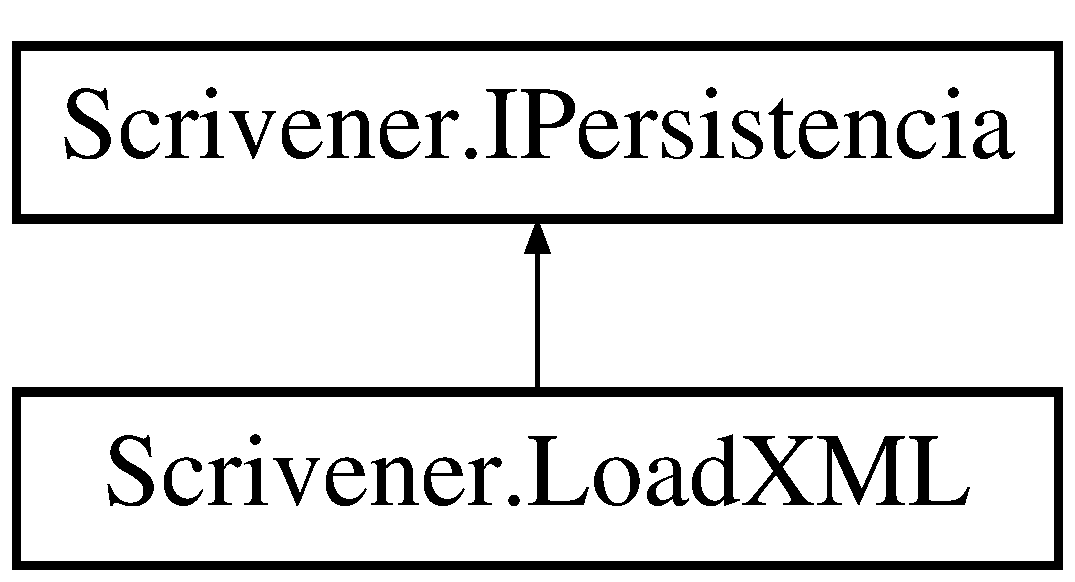
\includegraphics[height=2.000000cm]{interface_scrivener_1_1_i_persistencia}
\end{center}
\end{figure}
\subsection*{Public Member Functions}
\begin{DoxyCompactItemize}
\item 
Libro \hyperlink{interface_scrivener_1_1_i_persistencia_af261542f2a58e61e176ba2f74316e597}{Leer} ()
\end{DoxyCompactItemize}


\subsection{Detailed Description}


Definition at line 5 of file I\-Persistencia.\-cs.



\subsection{Member Function Documentation}
\hypertarget{interface_scrivener_1_1_i_persistencia_af261542f2a58e61e176ba2f74316e597}{\index{Scrivener\-::\-I\-Persistencia@{Scrivener\-::\-I\-Persistencia}!Leer@{Leer}}
\index{Leer@{Leer}!Scrivener::IPersistencia@{Scrivener\-::\-I\-Persistencia}}
\subsubsection[{Leer}]{\setlength{\rightskip}{0pt plus 5cm}Libro Scrivener.\-I\-Persistencia.\-Leer (
\begin{DoxyParamCaption}
{}
\end{DoxyParamCaption}
)}}\label{interface_scrivener_1_1_i_persistencia_af261542f2a58e61e176ba2f74316e597}


Implemented in \hyperlink{class_scrivener_1_1_load_x_m_l_ae5c0e87f3f365e244d01376501347f6e}{Scrivener.\-Load\-X\-M\-L}.



The documentation for this interface was generated from the following file\-:\begin{DoxyCompactItemize}
\item 
\hyperlink{_i_persistencia_8cs}{I\-Persistencia.\-cs}\end{DoxyCompactItemize}

\hypertarget{class_scrivener_1_1_load_x_m_l}{\section{Scrivener.\-Load\-X\-M\-L Class Reference}
\label{class_scrivener_1_1_load_x_m_l}\index{Scrivener.\-Load\-X\-M\-L@{Scrivener.\-Load\-X\-M\-L}}
}


Cargar archivo X\-M\-L  


Inheritance diagram for Scrivener.\-Load\-X\-M\-L\-:\begin{figure}[H]
\begin{center}
\leavevmode
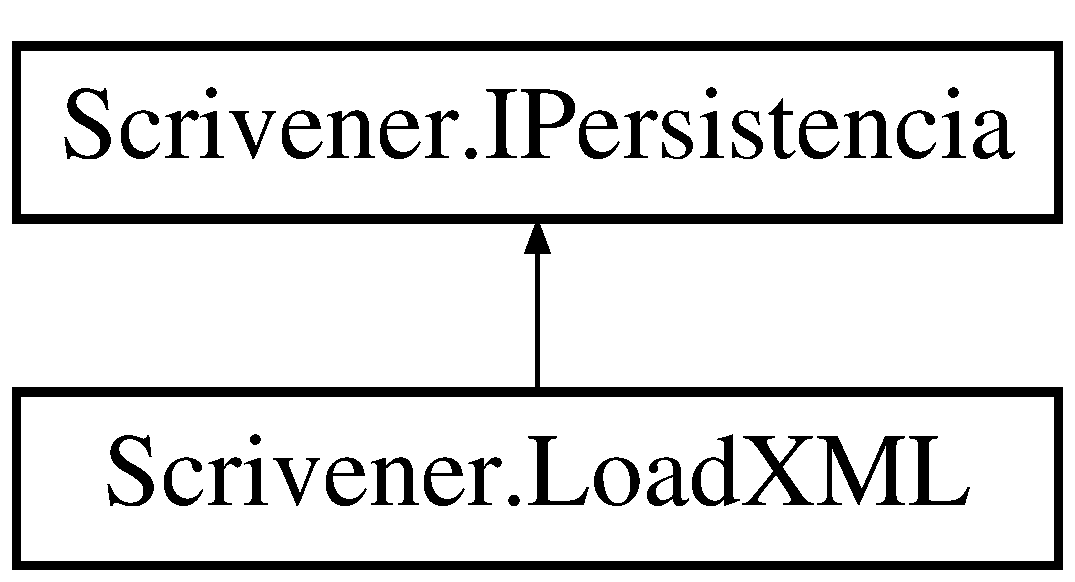
\includegraphics[height=2.000000cm]{class_scrivener_1_1_load_x_m_l}
\end{center}
\end{figure}
\subsection*{Public Member Functions}
\begin{DoxyCompactItemize}
\item 
\hyperlink{class_scrivener_1_1_load_x_m_l_aaac25883a7f3f34e585973ceff34238d}{Load\-X\-M\-L} (string documento)
\item 
Libro \hyperlink{class_scrivener_1_1_load_x_m_l_ae5c0e87f3f365e244d01376501347f6e}{Leer} ()
\begin{DoxyCompactList}\small\item\em Implementa el metodo principal de \hyperlink{class_scrivener_1_1_load_x_m_l}{Scrivener.\-Load\-X\-M\-L} con el que se carga en memoria un fichero \char`\"{}datos\-\_\-scrivener.\-xml\char`\"{} que contiene los datos sobre los capitulos del libro. \end{DoxyCompactList}\end{DoxyCompactItemize}


\subsection{Detailed Description}
Cargar archivo X\-M\-L 



Definition at line 10 of file Load\-X\-M\-L.\-cs.



\subsection{Constructor \& Destructor Documentation}
\hypertarget{class_scrivener_1_1_load_x_m_l_aaac25883a7f3f34e585973ceff34238d}{\index{Scrivener\-::\-Load\-X\-M\-L@{Scrivener\-::\-Load\-X\-M\-L}!Load\-X\-M\-L@{Load\-X\-M\-L}}
\index{Load\-X\-M\-L@{Load\-X\-M\-L}!Scrivener::LoadXML@{Scrivener\-::\-Load\-X\-M\-L}}
\subsubsection[{Load\-X\-M\-L}]{\setlength{\rightskip}{0pt plus 5cm}Scrivener.\-Load\-X\-M\-L.\-Load\-X\-M\-L (
\begin{DoxyParamCaption}
\item[{string}]{documento}
\end{DoxyParamCaption}
)}}\label{class_scrivener_1_1_load_x_m_l_aaac25883a7f3f34e585973ceff34238d}


Definition at line 12 of file Load\-X\-M\-L.\-cs.



\subsection{Member Function Documentation}
\hypertarget{class_scrivener_1_1_load_x_m_l_ae5c0e87f3f365e244d01376501347f6e}{\index{Scrivener\-::\-Load\-X\-M\-L@{Scrivener\-::\-Load\-X\-M\-L}!Leer@{Leer}}
\index{Leer@{Leer}!Scrivener::LoadXML@{Scrivener\-::\-Load\-X\-M\-L}}
\subsubsection[{Leer}]{\setlength{\rightskip}{0pt plus 5cm}Libro Scrivener.\-Load\-X\-M\-L.\-Leer (
\begin{DoxyParamCaption}
{}
\end{DoxyParamCaption}
)}}\label{class_scrivener_1_1_load_x_m_l_ae5c0e87f3f365e244d01376501347f6e}


Implementa el metodo principal de \hyperlink{class_scrivener_1_1_load_x_m_l}{Scrivener.\-Load\-X\-M\-L} con el que se carga en memoria un fichero \char`\"{}datos\-\_\-scrivener.\-xml\char`\"{} que contiene los datos sobre los capitulos del libro. 



Implements \hyperlink{interface_scrivener_1_1_i_persistencia_af261542f2a58e61e176ba2f74316e597}{Scrivener.\-I\-Persistencia}.



Definition at line 22 of file Load\-X\-M\-L.\-cs.



The documentation for this class was generated from the following file\-:\begin{DoxyCompactItemize}
\item 
\hyperlink{_load_x_m_l_8cs}{Load\-X\-M\-L.\-cs}\end{DoxyCompactItemize}

\hypertarget{class_scrivener_1_1_main_class}{\section{Scrivener.\-Main\-Class Class Reference}
\label{class_scrivener_1_1_main_class}\index{Scrivener.\-Main\-Class@{Scrivener.\-Main\-Class}}
}
\subsection*{Static Public Member Functions}
\begin{DoxyCompactItemize}
\item 
static void \hyperlink{class_scrivener_1_1_main_class_a9f612b59e2b2fb7e237e988d706f1941}{Main} (string\mbox{[}$\,$\mbox{]} args)
\end{DoxyCompactItemize}


\subsection{Detailed Description}


Definition at line 10 of file App.\-cs.



\subsection{Member Function Documentation}
\hypertarget{class_scrivener_1_1_main_class_a9f612b59e2b2fb7e237e988d706f1941}{\index{Scrivener\-::\-Main\-Class@{Scrivener\-::\-Main\-Class}!Main@{Main}}
\index{Main@{Main}!Scrivener::MainClass@{Scrivener\-::\-Main\-Class}}
\subsubsection[{Main}]{\setlength{\rightskip}{0pt plus 5cm}static void Scrivener.\-Main\-Class.\-Main (
\begin{DoxyParamCaption}
\item[{string\mbox{[}$\,$\mbox{]}}]{args}
\end{DoxyParamCaption}
)\hspace{0.3cm}{\ttfamily [static]}}}\label{class_scrivener_1_1_main_class_a9f612b59e2b2fb7e237e988d706f1941}


Definition at line 12 of file App.\-cs.



The documentation for this class was generated from the following file\-:\begin{DoxyCompactItemize}
\item 
\hyperlink{_app_8cs}{App.\-cs}\end{DoxyCompactItemize}

\hypertarget{class_scrivener_1_1_user_interface}{\section{Scrivener.\-User\-Interface Class Reference}
\label{class_scrivener_1_1_user_interface}\index{Scrivener.\-User\-Interface@{Scrivener.\-User\-Interface}}
}
Inheritance diagram for Scrivener.\-User\-Interface\-:\begin{figure}[H]
\begin{center}
\leavevmode
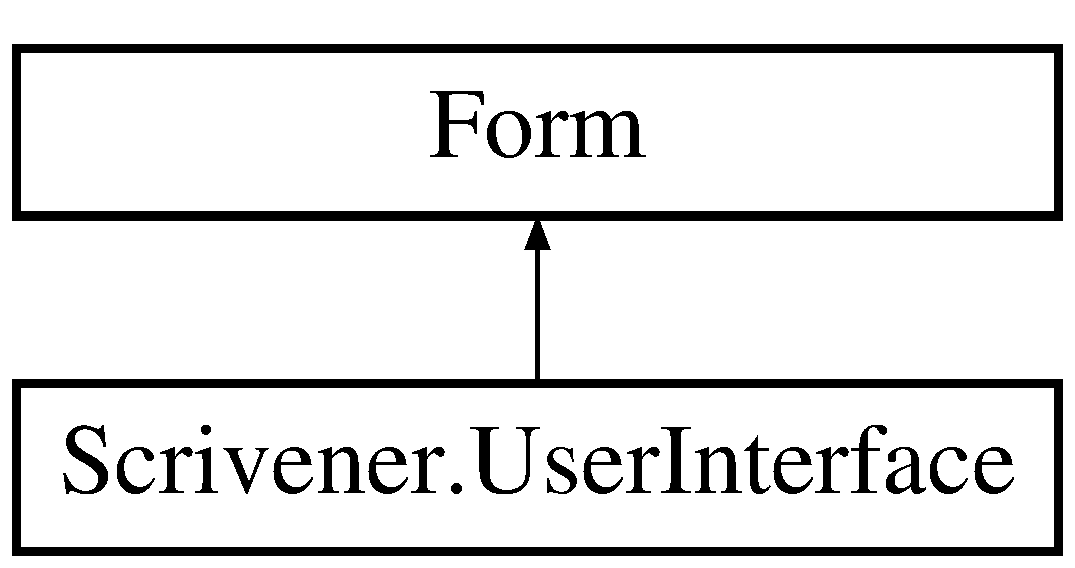
\includegraphics[height=2.000000cm]{class_scrivener_1_1_user_interface}
\end{center}
\end{figure}
\subsection*{Public Member Functions}
\begin{DoxyCompactItemize}
\item 
\hyperlink{class_scrivener_1_1_user_interface_a2530c43ebdb8eb24c279ccf4ef03f62d}{User\-Interface} (\hyperlink{interface_scrivener_1_1_i_persistencia}{I\-Persistencia} object\-Persistencia, Panel panel)
\item 
void \hyperlink{class_scrivener_1_1_user_interface_a50dc5329e3dab19828d1007bdaafdb45}{Build\-Gui} ()
\end{DoxyCompactItemize}
\subsection*{Properties}
\begin{DoxyCompactItemize}
\item 
\hyperlink{interface_scrivener_1_1_i_persistencia}{I\-Persistencia} \hyperlink{class_scrivener_1_1_user_interface_a4029948a0c4bb3d5c6407872ac9ea878}{Object\-Persistencia}\hspace{0.3cm}{\ttfamily  \mbox{[}get, set\mbox{]}}
\begin{DoxyCompactList}\small\item\em Gets y sets de la propiedad Object\-Persistencia. \end{DoxyCompactList}\end{DoxyCompactItemize}


\subsection{Detailed Description}


Definition at line 8 of file User\-Interface.\-cs.



\subsection{Constructor \& Destructor Documentation}
\hypertarget{class_scrivener_1_1_user_interface_a2530c43ebdb8eb24c279ccf4ef03f62d}{\index{Scrivener\-::\-User\-Interface@{Scrivener\-::\-User\-Interface}!User\-Interface@{User\-Interface}}
\index{User\-Interface@{User\-Interface}!Scrivener::UserInterface@{Scrivener\-::\-User\-Interface}}
\subsubsection[{User\-Interface}]{\setlength{\rightskip}{0pt plus 5cm}Scrivener.\-User\-Interface.\-User\-Interface (
\begin{DoxyParamCaption}
\item[{{\bf I\-Persistencia}}]{object\-Persistencia, }
\item[{Panel}]{panel}
\end{DoxyParamCaption}
)}}\label{class_scrivener_1_1_user_interface_a2530c43ebdb8eb24c279ccf4ef03f62d}


Definition at line 10 of file User\-Interface.\-cs.



\subsection{Member Function Documentation}
\hypertarget{class_scrivener_1_1_user_interface_a50dc5329e3dab19828d1007bdaafdb45}{\index{Scrivener\-::\-User\-Interface@{Scrivener\-::\-User\-Interface}!Build\-Gui@{Build\-Gui}}
\index{Build\-Gui@{Build\-Gui}!Scrivener::UserInterface@{Scrivener\-::\-User\-Interface}}
\subsubsection[{Build\-Gui}]{\setlength{\rightskip}{0pt plus 5cm}void Scrivener.\-User\-Interface.\-Build\-Gui (
\begin{DoxyParamCaption}
{}
\end{DoxyParamCaption}
)}}\label{class_scrivener_1_1_user_interface_a50dc5329e3dab19828d1007bdaafdb45}


Definition at line 18 of file User\-Interface.\-cs.



\subsection{Property Documentation}
\hypertarget{class_scrivener_1_1_user_interface_a4029948a0c4bb3d5c6407872ac9ea878}{\index{Scrivener\-::\-User\-Interface@{Scrivener\-::\-User\-Interface}!Object\-Persistencia@{Object\-Persistencia}}
\index{Object\-Persistencia@{Object\-Persistencia}!Scrivener::UserInterface@{Scrivener\-::\-User\-Interface}}
\subsubsection[{Object\-Persistencia}]{\setlength{\rightskip}{0pt plus 5cm}{\bf I\-Persistencia} Scrivener.\-User\-Interface.\-Object\-Persistencia\hspace{0.3cm}{\ttfamily [get]}, {\ttfamily [set]}}}\label{class_scrivener_1_1_user_interface_a4029948a0c4bb3d5c6407872ac9ea878}


Gets y sets de la propiedad Object\-Persistencia. 

Objeto que proporciona los metodos para actualizar tree\-View nuevos datos. 

Definition at line 114 of file User\-Interface.\-cs.



The documentation for this class was generated from the following file\-:\begin{DoxyCompactItemize}
\item 
\hyperlink{_user_interface_8cs}{User\-Interface.\-cs}\end{DoxyCompactItemize}

\chapter{File Documentation}
\hypertarget{_app_8cs}{\section{App.\-cs File Reference}
\label{_app_8cs}\index{App.\-cs@{App.\-cs}}
}
\subsection*{Classes}
\begin{DoxyCompactItemize}
\item 
class \hyperlink{class_scrivener_1_1_main_class}{Scrivener.\-Main\-Class}
\end{DoxyCompactItemize}
\subsection*{Namespaces}
\begin{DoxyCompactItemize}
\item 
package \hyperlink{namespace_scrivener}{Scrivener}
\end{DoxyCompactItemize}

\hypertarget{_assembly_info_8cs}{\section{Assembly\-Info.\-cs File Reference}
\label{_assembly_info_8cs}\index{Assembly\-Info.\-cs@{Assembly\-Info.\-cs}}
}

\hypertarget{_i_persistencia_8cs}{\section{I\-Persistencia.\-cs File Reference}
\label{_i_persistencia_8cs}\index{I\-Persistencia.\-cs@{I\-Persistencia.\-cs}}
}
\subsection*{Classes}
\begin{DoxyCompactItemize}
\item 
interface \hyperlink{interface_scrivener_1_1_i_persistencia}{Scrivener.\-I\-Persistencia}
\end{DoxyCompactItemize}
\subsection*{Namespaces}
\begin{DoxyCompactItemize}
\item 
package \hyperlink{namespace_scrivener}{Scrivener}
\end{DoxyCompactItemize}

\hypertarget{_load_x_m_l_8cs}{\section{Load\-X\-M\-L.\-cs File Reference}
\label{_load_x_m_l_8cs}\index{Load\-X\-M\-L.\-cs@{Load\-X\-M\-L.\-cs}}
}
\subsection*{Classes}
\begin{DoxyCompactItemize}
\item 
class \hyperlink{class_scrivener_1_1_load_x_m_l}{Scrivener.\-Load\-X\-M\-L}
\begin{DoxyCompactList}\small\item\em Cargar archivo X\-M\-L \end{DoxyCompactList}\end{DoxyCompactItemize}
\subsection*{Namespaces}
\begin{DoxyCompactItemize}
\item 
package \hyperlink{namespace_scrivener}{Scrivener}
\end{DoxyCompactItemize}

\hypertarget{_user_interface_8cs}{\section{User\-Interface.\-cs File Reference}
\label{_user_interface_8cs}\index{User\-Interface.\-cs@{User\-Interface.\-cs}}
}
\subsection*{Classes}
\begin{DoxyCompactItemize}
\item 
class \hyperlink{class_scrivener_1_1_user_interface}{Scrivener.\-User\-Interface}
\end{DoxyCompactItemize}
\subsection*{Namespaces}
\begin{DoxyCompactItemize}
\item 
package \hyperlink{namespace_scrivener}{Scrivener}
\end{DoxyCompactItemize}

%--- End generated contents ---

% Index
\newpage
\phantomsection
\addcontentsline{toc}{part}{Index}
\printindex

\end{document}
